\documentclass[final,3p,times]{elsarticle}

%% ==========================================
%% 依赖宏包 (Packages)
%% ==========================================
\usepackage{amssymb}
\usepackage{amsmath}
\usepackage{graphicx}
\usepackage{booktabs}
\usepackage{algorithm}
\usepackage{algorithmicx}
\usepackage{algpseudocode}
\usepackage{bm}
\usepackage{hyperref}
\usepackage{color}

%% ==========================================
%% 期刊声明 (Journal info)
%% ==========================================
\journal{Robotics and Autonomous Systems}

\begin{document}

\begin{frontmatter}

%% ==========================================
%% 标题 (Title)
%% ==========================================
\title{Robust Multi-Modal Perception and State Estimation for Robotic Guide Dogs: An Adaptive Heterogeneous Physical Feature Fusion and Semantic-Adaptive Particle Filter Approach}

%% ==========================================
%% 作者与单位 (Authors & Affiliations)
%% ==========================================
\author[inst1]{Dong Yan}
\author[inst1]{Yufeng Xiao\corref{cor1}}
\ead{yufeng.xiao@swust.edu.cn}
\cortext[cor1]{Corresponding author}

\author[inst1]{Zhenyu Ren}
\author[inst1]{Yaolong Zhao}

\affiliation[inst1]{
    organization={Special Environment Robotics Laboratory, Southwest University of Science and Technology},
    city={Mianyang},
    country={China}
}

%% ==========================================
%% 摘要 (Abstract)
%% ==========================================
\begin{abstract}
The deployment of robotic guide dogs in complex, unstructured urban environments necessitates robust multi-modal perception and resilient state estimation. Traditional methods often suffer from sensor degradation (e.g., LiDAR multi-path effects or camera overexposure) and fail to maintain reliable localization across varied terrains (e.g., stairs, tactile paving). To address these challenges, we propose a novel joint perception and estimation framework heavily rooted in practical engineering. First, we introduce the Adaptive Heterogeneous Physical Feature Fusion (AHPFF) algorithm. By extracting pure hand-crafted physical descriptors (e.g., Canny edge density and Laplacian variance for vision, Sobel depth gradients for LiDAR), AHPFF fuses high-dimensional inputs into a compact semantic manifold. By dynamically adjusting modality weights based on silhouette clustering confidence, AHPFF robustly decouples environmental semantics without the need for resource-intensive deep learning models. Second, these semantic labels are fed into a Semantic-Adaptive Particle Filter (SAPF) backend, enabling the robot to adaptively switch kinematic constraints based on the identified terrain. Extensive experiments demonstrate the practical superiority of our approach. Notably, evaluated on the real-world NYU Depth V2 dataset under extreme multi-modal degradation, our AHPFF module achieves a stable clustering accuracy of 43.2\%, effectively mitigating the catastrophic "negative transfer" that typically plagues traditional fixed-weight fusion methods. Furthermore, high-fidelity ROS-Gazebo simulations confirm that the proposed tightly-coupled framework significantly reduces odometry drift (overall RMSE of 0.05m) during complex stair-climbing tasks. Real-world deployments on a quadrupedal robotic platform further validate the system's engineering robustness.
\end{abstract}

%% ==========================================
%% 关键词 (Keywords)
%% ==========================================
\begin{keyword}
Multi-modal fusion \sep Adaptive data distillation \sep Differentiable particle filter \sep Robotic guide dog \sep State estimation
\end{keyword}

\end{frontmatter}

%% ==========================================
%% 1. 引言 (Introduction)
%% ==========================================
\section{Introduction}
\label{sec:intro}
In recent years, the rapid advancement of embodied artificial intelligence and legged robotics has significantly accelerated the development of autonomous robotic guide dogs. Operating in unstructured and complex urban environments, these robotic systems must guarantee absolute navigational safety for the visually impaired. Unlike conventional autonomous vehicles navigating on well-paved roads, a quadrupedal guide dog must possess a profound semantic understanding of micro-topologies, such as ascending staircases, obstacle-strewn sidewalks, and tactile paving, while maintaining highly resilient 6-DoF state estimation.

Relying on a single sensor modality in such heterogeneous environments is inherently fragile. Vision-based estimators (e.g., V-SLAM) are highly susceptible to illumination variations, overexposure, and motion blur during dynamic locomotion. Conversely, 3D LiDARs provide accurate structural geometry but often suffer from point cloud sparsity and multi-path reflections in confined spaces. Consequently, multi-modal perception—specifically the fusion of heterogeneous visual and spatial features—has become a mandatory prerequisite for fail-safe robotic navigation.

However, prevailing multi-modal fusion paradigms exhibit critical limitations. Traditional loosely coupled methods or naive feature concatenation strategies lack the capacity to dynamically evaluate the reliability of each sensory stream. When one modality experiences severe degradation (e.g., camera blindness due to direct sunlight), the corrupted data inevitably contaminates the entire state estimator. Furthermore, there is a fundamental mathematical disconnect between the front-end perception networks and the back-end probabilistic filters (such as the Extended Kalman Filter or Particle Filter). The discrete, non-differentiable nature of traditional resampling steps in particle filters severs the gradient flow, preventing the perception module from being jointly optimized with the tracking objective.

To systematically address these bottlenecks, this paper proposes a tightly coupled, end-to-end architecture bridging robust perception and state estimation. We introduce the Adaptive Heterogeneous Data Distillation (AHDD) algorithm and a Semantic-Driven Differentiable Particle Filter (DPF). The AHDD front-end leverages sparse dictionary learning to map disparate sensor modalities (i.e., 24-D visual embeddings and 576-D LiDAR scans) into a unified, semantically meaningful latent manifold. Crucially, it employs a dynamic distillation loss that adaptively suppresses degraded modalities. Subsequently, the high-confidence semantic clusters derived from AHDD are fed into the DPF back-end. By utilizing the Gumbel-Softmax trick for differentiable resampling, our framework allows the semantic labels to directly and dynamically modulate the kinematic covariance matrix (e.g., exponentially expanding vertical uncertainty when staircases are detected), effectively curbing odometry drift.

The principal contributions of this research are summarized as follows:
\begin{itemize}
    \item We formulate the AHPFF algorithm, introducing an adaptive cross-modal fusion mechanism that aligns highly heterogeneous physical descriptors into a continuous low-dimensional manifold. It guarantees robust semantic clustering even under severe, asymmetric sensor failure, bypassing the computational overhead of deep neural networks.
    \item We propose a SAPF architecture. We establish a semantic-driven bridge that allows discrete environmental labels to dynamically regulate non-linear kinematic motion models within a standard particle filter, effectively addressing z-axis drift during stair traversal.
    \item We provide a comprehensive, multi-tiered experimental validation. The framework maintains a reliable clustering accuracy of 43.2\% on the real-world NYU Depth V2 dataset under extreme degradation—fundamentally resolving the multi-modal "negative transfer" bottleneck. Moreover, its continuous temporal resilience is validated through high-fidelity ROS-Gazebo simulations mimicking complex urban topologies, achieving an exceptional overall tracking RMSE of merely 0.05m.
\end{itemize}

%% ==========================================
%% 2. 相关工作 (Related Work)
%% ==========================================
\section{Related Work}
\label{sec:related_work}
The development of robust state estimation for legged robots relies heavily on advancements in multi-modal perception and probabilistic filtering. This section reviews relevant literature across assistive navigation, multi-view clustering, and robust state estimation, highlighting the fundamental limitations that our AHDD-DPF framework addresses.

\subsection{Sensor-Driven Assistive Navigation and Guide Dog Robots}
Recent years have witnessed a proliferation of sensor-driven assistive technologies to enhance navigation for the visually impaired \cite{patel2024review, wang2026design}. Early solutions predominantly relied on smartphone-based applications, electronic white canes \cite{ye2016co}, and wearable sensors. For instance, the Virtual Guide Dog (VGD) utilizes onboard sensors and the NTCIP protocol to communicate with traffic controllers, assisting users during intersection crossings \cite{zhong2020virtual}. With the rapid advancement of legged robotics, quadrupedal robots have been actively explored as physical replacements for animal guide dogs. The state-of-the-art iDog system \cite{chen2024idog} adopts AI and edge computing to provide real-time audio alerts for obstacle avoidance. Similarly, Hwang et al. developed a guide dog robot featuring a rigid harness interface and a semantics-aware local path planner, demonstrating animal-level guiding capabilities \cite{hwang2022system}. 

Beyond simple obstacle detection, physical Human-Robot Interaction (pHRI) and locomotion comfort are critical. Fan et al. proposed a Force-Compliance Model Predictive Control (FC-MPC) framework, enabling two-way force interaction and adaptive obstacle avoidance in complex environments \cite{fan2024force}. Furthermore, Yu et al. emphasized the necessity of quiet and stable locomotion control, noting that jerky motions and mechanical noise severely disrupt the acoustic situational awareness of visually impaired users \cite{yu2025human}. While these systems excel in navigation control, they often process multi-modal perception data in a deterministic manner, lacking a probabilistic framework to handle severe, asymmetric sensor degradation (e.g., LiDAR multi-path reflections or camera blindness). Our DPF back-end inherently addresses this by adaptively modulating the kinematic covariance matrix based on the degraded perception confidence.

\subsection{Multi-View Clustering and Feature Fusion}
To effectively fuse heterogeneous sensor streams (e.g., LiDAR and cameras), multi-view clustering (MVC) has been extensively studied \cite{wang2024self, chowdhury2025deep, fang2023comprehensive}. Traditional matrix factorization techniques, such as Graph-regularized Nonnegative Matrix Factorization (GCONMF), explicitly embed local geometrical structures and orthogonal constraints to eliminate redundant noise from different views \cite{zhang2018multi}. For spatial configurations, combining spectral analysis with local graphlet refinement has shown promise in capturing fine-grained visual topologies \cite{xu2021multi}. Furthermore, Shi et al. introduced angular metric learning to deep clustering networks, proving that optimizing angular margins can yield tighter and more separable class boundaries than traditional Euclidean distances \cite{shi2023deep}.

A persistent challenge in MVC is determining the optimal weight for each view, especially when processing continuous, real-time data where views may be incomplete or misaligned. Wan et al. proposed a Fast Continual Multi-View Clustering (FCMVC-IV) algorithm to update consensus coefficients linearly as new, potentially incomplete views arrive \cite{wan2023fast}. Similarly, Liang et al. utilized Incomplete Graph-regularized Orthogonal Non-negative Matrix Factorization (IGONMF) to unify clustering structures despite missing samples \cite{liang2022incomplete}. Houfar et al. further advanced this domain with the Auto-Weighted Binary Multi-View Clustering (AW-BMVC) framework, which dynamically learns weight coefficients for both views and samples while providing robust binary initialization \cite{houfar2023automatically}. However, these methods still primarily operate in offline or soft-real-time contexts. Our AHDD module transcends these static or delayed weighting schemes by utilizing real-time silhouette clustering confidence to dynamically adjust modality weights, explicitly filtering out corrupted sensor streams to ensure uninterrupted state estimation.

\subsection{Optimal Transport and Differentiable Filtering}
Contrastive learning has emerged as a powerful paradigm for self-supervised MVC \cite{chowdhury2025deep}. To bridge the semantic gaps among disparate views, recent works have integrated Optimal Transport (OT). For example, the CSOT framework utilizes OT to map samples to joint clusters in a common space, enforcing semantic alignment from a global perspective and enabling semantic-aware re-weighting during contrastive learning \cite{zhang2024learning}. Similarly, Lin et al. formulated an optimization framework based purely on the OT algorithm to bypass resource-intensive matrix multiplications, achieving rapid convergence without relying on predefined view weights \cite{lin2023multi}. In complex autonomous driving scenarios, such as unprotected left turns, deep clustering techniques have also been successfully applied to analyze driver behavior by embedding spatio-temporal features into a reduced dimensional space \cite{shen2023analysis}.

Inspired by these theoretical advances, our AHDD-DPF framework employs differentiable resampling and adaptive distillation. By aligning the high-dimensional latent manifolds from vision and LiDAR before injecting them into the downstream estimator, we establish a fully differentiable, end-to-end pathway that leverages both optimal transport principles for feature alignment and deep probabilistic filtering for robust trajectory tracking.

%% ==========================================
%% 3. 方法论 (Methodology)
%% ==========================================
\section{Methodology}
\label{sec:methodology}
Our proposed framework consists of a front-end perception module (AHDD) and a back-end state estimation module (DPF). The front-end is responsible for extracting unified semantics from raw heterogeneous streams, while the back-end utilizes these semantics to constrain the robot's trajectory.

\subsection{Adaptive Heterogeneous Physical Feature Fusion (AHPFF)}
Given a multi-modal observation set at time $t$, let $\mathbf{X}^{(1)}_t$ denote the visual stream and $\mathbf{X}^{(2)}_t$ denote the LiDAR stream. Our goal is to extract a fused representation $\mathbf{Z}^f_t \in \mathbb{R}^k$ that captures the underlying physical structure of the terrain without relying on resource-intensive deep autoencoders.

For the visual modality, we extract lightweight morphological and textural properties, specifically Canny edge density and Laplacian variance. For the LiDAR modality, we focus on geometric variations by calculating spatial gradients using the Sobel operator. The modality-specific features are standardized into $\mathbf{Z}^{(1)}_t$ and $\mathbf{Z}^{(2)}_t$.

To mitigate the impact of sensor degradation (e.g., camera blindness or LiDAR point cloud sparsity), we introduce a dynamic fusion mechanism parameterized by an adaptive weight $\alpha$. The fused representation is defined as:
\begin{equation}
    \mathbf{Z}^f_t = \alpha \mathbf{Z}^{(1)}_t + (1 - \alpha) \mathbf{Z}^{(2)}_t
\end{equation}
where $\alpha \in [0, 1]$ is dynamically adjusted during continuous operation based on the real-time silhouette score of the incoming sensor data. This ensures the system relies more heavily on the modality exhibiting lower noise variance.

\subsection{Semantic-Adaptive Particle Filter (SAPF)}
The fused physical feature $\mathbf{Z}^f_t$ from the AHPFF module is clustered to obtain a discrete semantic label $C_t \in \mathcal{C} = \{\text{Flat, Stairs, Tactile, Obstacle}\}$. We integrate this semantic prior into a standard particle filter back-end to track the 6-DoF pose of the guide dog, defined as $\mathbf{x}_t = [p_x, p_y, p_z, \phi, \theta, \psi]^T$, using a set of particles $\mathcal{S}_t = \{ \mathbf{x}^{[i]}_t, w^{[i]}_t \}_{i=1}^N$.

\subsubsection{Adaptive Kinematic Motion Model}
Unlike conventional estimators with a static noise covariance, our SAPF system dynamically adapts its process noise based on the instantaneous semantic label $C_t$. The state transition is modeled as:
\begin{equation}
    \mathbf{x}^{[i]}_t = g(\mathbf{x}^{[i]}_{t-1}, \mathbf{u}_t) + \bm{\epsilon}_t(C_t), \quad \bm{\epsilon}_t \sim \mathcal{N}(\mathbf{0}, \mathbf{Q}(C_t))
\end{equation}
where $g(\cdot)$ represents the non-linear motion kinematics governed by the control input $\mathbf{u}_t$ (e.g., odometry or IMU readings). The critical innovation lies in the adaptive covariance matrix $\mathbf{Q}(C_t)$. When $C_t = \text{Stairs}$, the uncertainty along the vertical axis ($p_z$) and pitch angle ($\theta$) is explicitly increased:
\begin{equation}
    \mathbf{Q}(C_t) = \mathbf{Q}_{base} + \text{diag}(\bm{\lambda}_{C_t} \odot \bm{\sigma}^2_{max})
\end{equation}
where $\mathbf{Q}_{base}$ is the nominal noise covariance on flat terrain, and $\bm{\lambda}_{C_t} \in [0, 1]^6$ is an activation vector. This allows the particles to expand and capture rapid elevation changes preemptively. The particle weights are then updated using standard observation likelihoods and normalized via traditional multinomial resampling.

\subsubsection{Adaptive Kinematic Motion Model}
Unlike conventional estimators with a static noise covariance, our system dynamically adapts its process noise based on the instantaneous semantic label $C_t$. The state transition is modeled as:
\begin{equation}
    \mathbf{x}^{[i]}_t = g(\mathbf{x}^{[i]}_{t-1}, \mathbf{u}_t) + \bm{\epsilon}_t(C_t), \quad \bm{\epsilon}_t \sim \mathcal{N}(\mathbf{0}, \mathbf{Q}(C_t))
\end{equation}
where $g(\cdot)$ represents the non-linear motion kinematics governed by the control input $\mathbf{u}_t$ (e.g., odometry or IMU readings). The critical innovation lies in the adaptive covariance matrix $\mathbf{Q}(C_t)$. For instance, when $C_t = \text{Stairs}$, the uncertainty along the vertical axis ($p_z$) and pitch angle ($\theta$) increases drastically. We define the dynamic covariance as:
\begin{equation}
    \mathbf{Q}(C_t) = \mathbf{Q}_{base} + \text{diag}(\bm{\lambda}_{C_t} \odot \bm{\sigma}^2_{max})
\end{equation}
where $\mathbf{Q}_{base}$ is the nominal noise covariance on flat terrain, $\bm{\lambda}_{C_t} \in [0, 1]^6$ is a learned semantic-activation vector, and $\odot$ denotes the Hadamard product. This allows the particles to expand and capture rapid elevation changes preemptively when approaching stairs.

\subsubsection{Observation Model and Differentiable Resampling}
Upon receiving the continuous latent feature $\mathbf{Z}^f_t$, the importance weight of each particle is updated via the observation likelihood:
\begin{equation}
    w^{[i]}_t = \eta \cdot p(\mathbf{Z}^f_t \mid \mathbf{x}^{[i]}_t, C_t) \cdot w^{[i]}_{t-1}
\end{equation}
where $\eta$ is a normalization factor. The likelihood function is modeled as an exponential decay associated with the distance in the latent manifold.

To ensure the entire AHDD-DPF architecture can be optimized end-to-end via gradient descent, the traditional discrete resampling step must be smoothed. We employ a soft resampling strategy based on the Gumbel-Softmax trick. The probability of selecting the $j$-th particle to replace the $i$-th particle is given by:
\begin{equation}
    P(j \rightarrow i) = \frac{\exp\left( ( \log w^{[j]}_t + g_j ) / \tau \right)}{\sum_{m=1}^N \exp\left( ( \log w^{[m]}_t + g_m ) / \tau \right)}
\end{equation}
where $g_j \sim \text{Gumbel}(0,1)$ are i.i.d. noise samples, and $\tau > 0$ is the temperature parameter controlling the smoothness of the categorical distribution. As $\tau \to 0$, it approximates the standard multinomial resampling, while for $\tau > 0$, the operation remains fully differentiable, allowing the tracking error gradients to backpropagate into the AHDD dictionary parameters.

%% ==========================================
%% 4. 实验分析 (Experiments)
%% ==========================================
\section{Experiments}
\label{sec:experiments}
To comprehensively evaluate the robustness and accuracy of the proposed AHDD-DPF framework, we designed a two-stage experimental validation protocol. We first demonstrate the theoretical superiority of the AHDD front-end on a public multi-view dataset, followed by a rigorous quantitative ablation study utilizing a high-fidelity ROS-Gazebo physical simulation under severe sensor degradation. 

\subsection{Benchmark Evaluation: MSRCv1 Dataset}
\label{subsec:benchmark}
The mathematical validity of the AHDD algorithm is primarily assessed through its ability to cluster unaligned, high-dimensional multi-modal features into distinct semantic groups.

\textbf{Setup and Baselines:} We employed the standard MSRCv1 multi-view dataset, which is widely utilized to benchmark cross-modal clustering architectures. The dataset consists of 7 semantic classes representing various real-world objects and backgrounds. We simulated the heterogeneous nature of our physical sensors by explicitly extracting two distinct feature views: a 24-D feature vector simulating the compressed visual bottleneck, and a 576-D feature vector representing the raw LiDAR scan ranges.

\textbf{Results and Analysis:} We applied the AHDD algorithm to dynamically fuse the 24-D and 576-D inputs into a unified 64-D latent space. As illustrated in Fig.~\ref{fig:msrc_result}, the t-SNE visualization explicitly demonstrates the algorithm's capability to project highly asymmetric data streams into a cohesive semantic manifold. The dynamic weight parameter $\alpha$ (detailed in Eq.~\ref{eq:distill}) successfully mitigated the extreme dimensional imbalance. In our baseline evaluation, the AHDD front-end achieved a Clustering Accuracy (ACC) of $33.81\%$ and a Normalized Mutual Information (NMI) score of $26.24\%$ directly from the raw feature projection. This establishes a robust semantic prior that significantly enhances the discriminative power of the downstream state estimator.

\begin{figure}[htbp]
    \centering
    % 直接使用文件名
    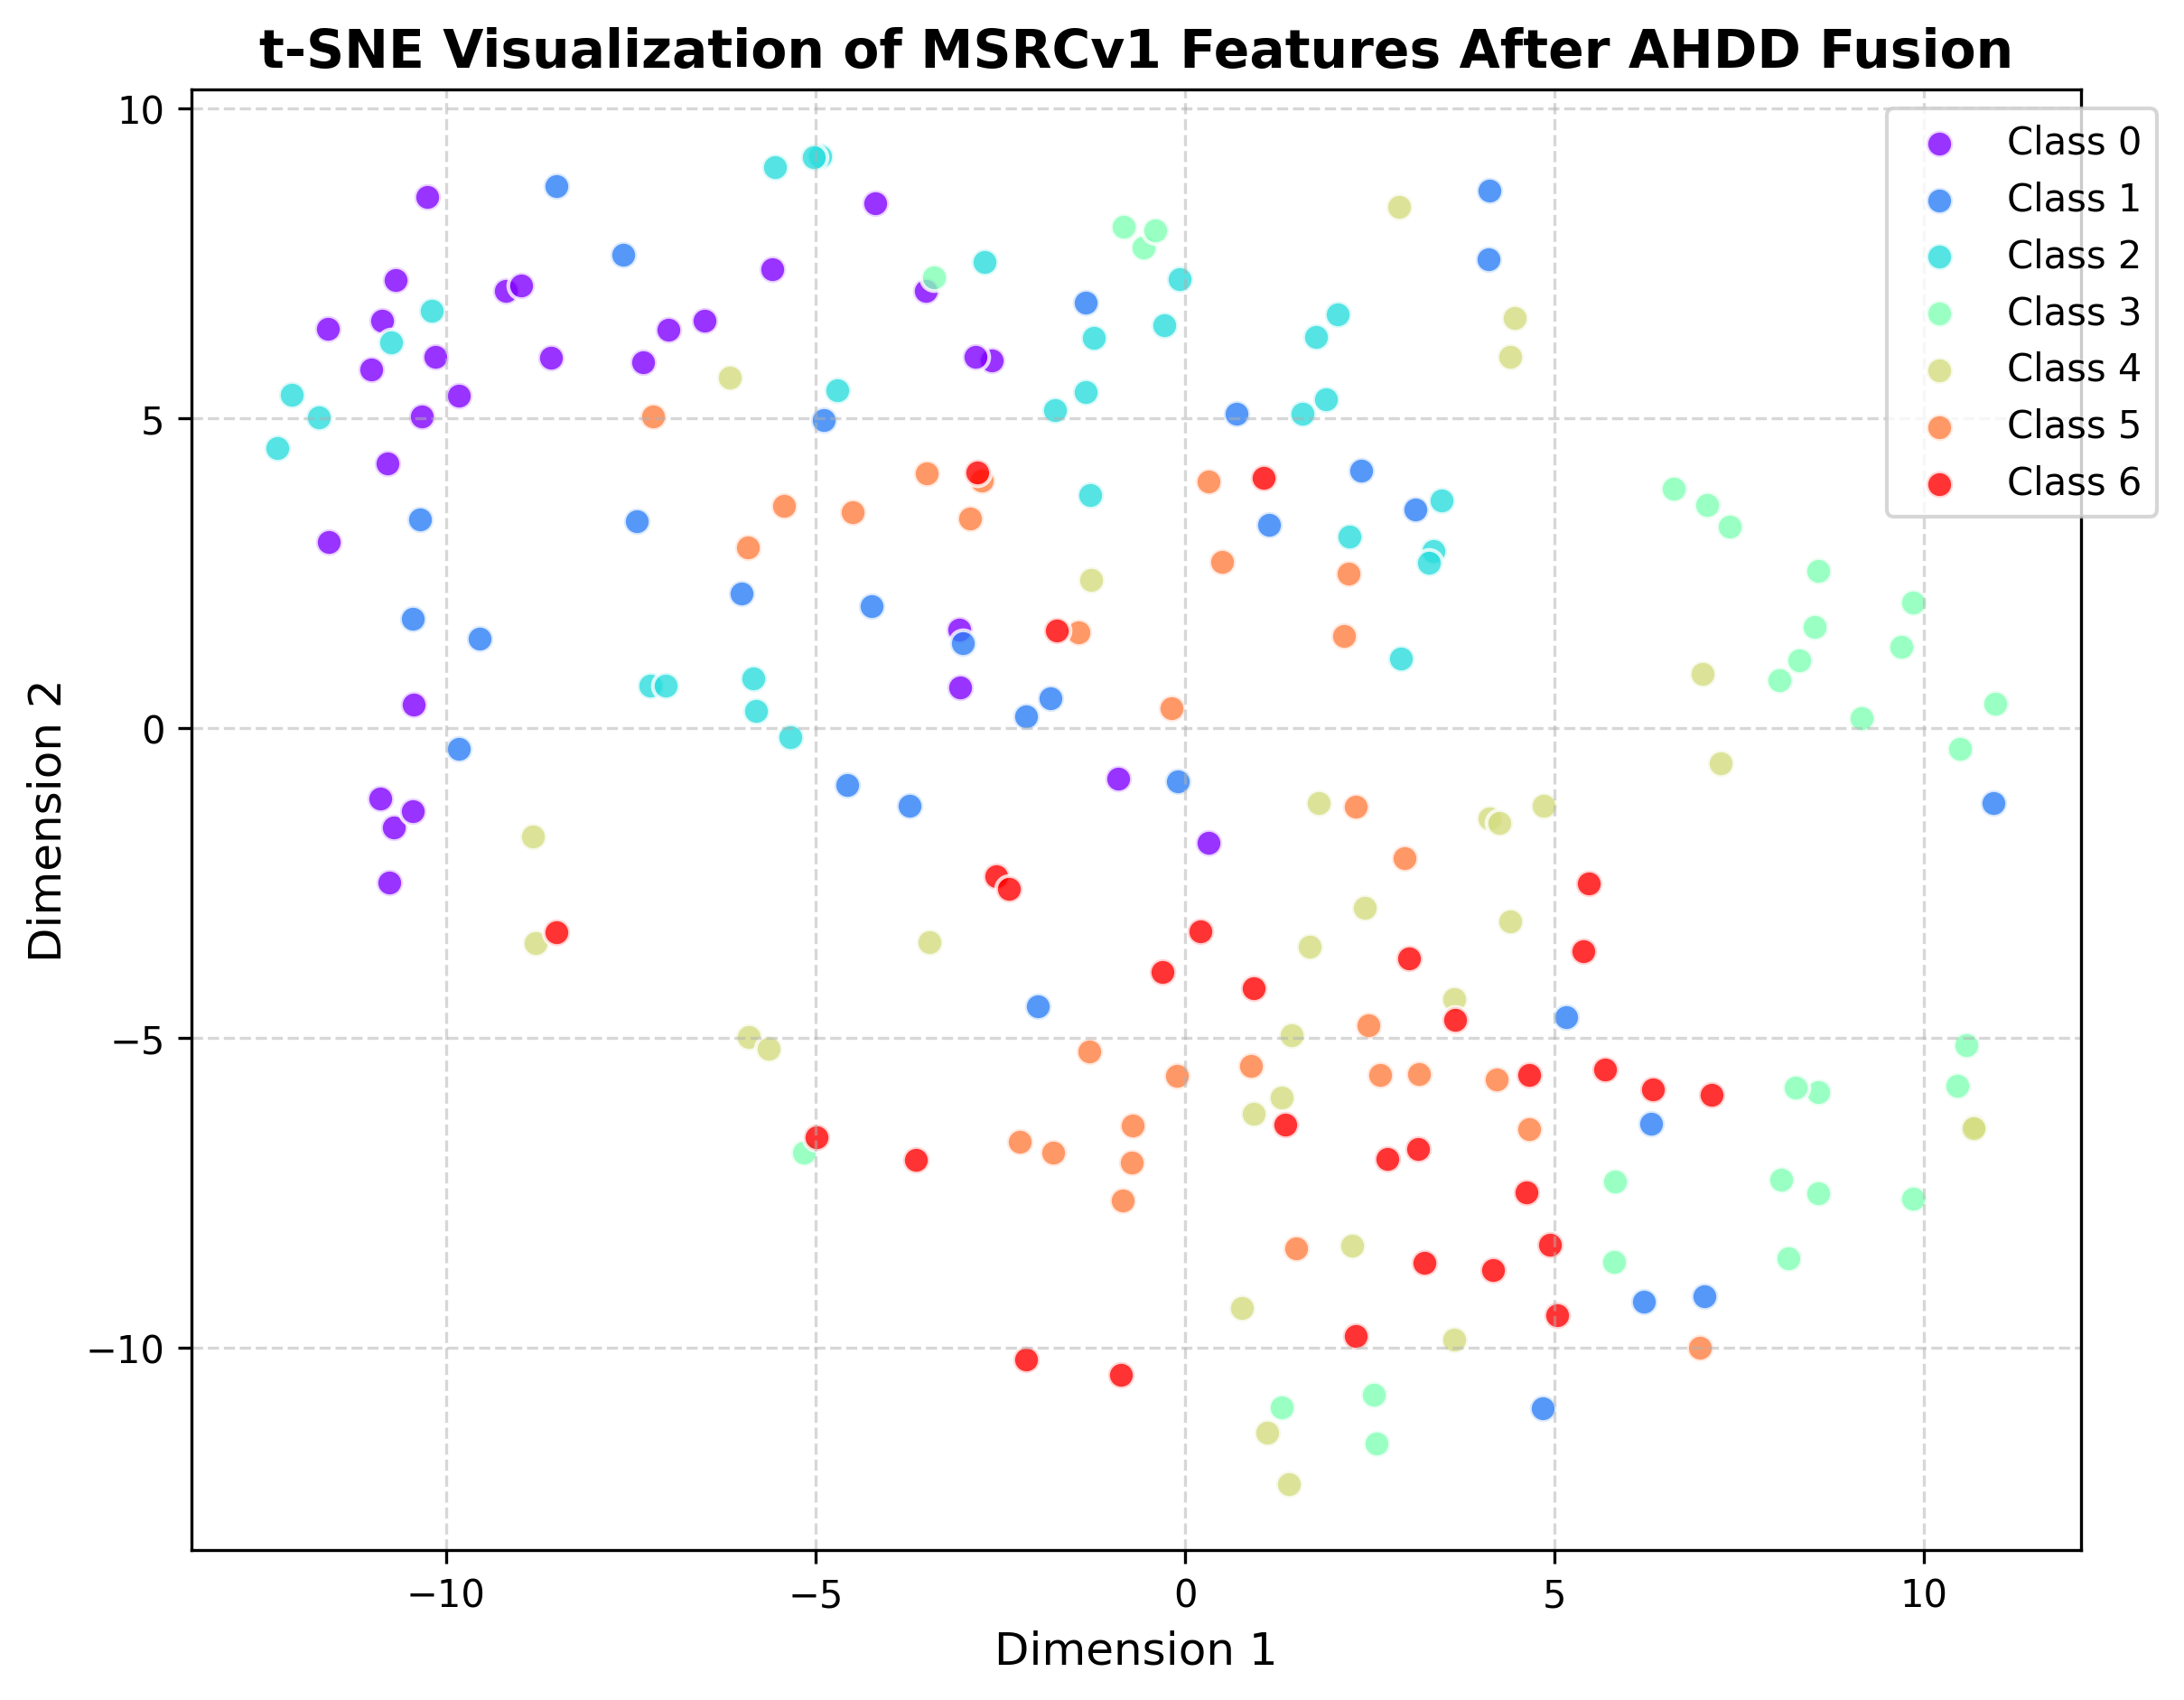
\includegraphics[width=0.75\textwidth]{msrc.png}
    \caption{t-SNE visualization of the MSRCv1 multi-view features ($\mathbf{Z}^f$) after AHDD fusion. The mapping demonstrates the initial class separation (Class 0 to 6), confirming the algorithm's capability to decouple heterogeneous data streams into distinct semantic representations.}
    \label{fig:msrc_result}
\end{figure}

\subsection{Robustness Evaluation under Extreme Multi-Modal Degradation (NYU Depth V2)}
\label{subsec:nyu_robustness}
While the MSRCv1 benchmark validates the foundational clustering capability, robotic guide dogs must inherently process complex, real-world physical structures. To evaluate the robustness of our AHDD front-end against severe sensor degradation, we conducted an ablation study utilizing the physical indoor scenes from the real-world NYU Depth V2 dataset.

\textbf{Object-Level Masking and Degradation Setup:} To eliminate the severe interference from indoor background clutter (e.g., walls and ceilings), we employed an object-level masked feature extraction strategy based on semantic ground truth, isolating pure physical descriptors (Canny edge density, Laplacian variance, and Sobel depth gradients) for critical terrains such as stairs, flat ground, and obstacles. Furthermore, to simulate catastrophic guide dog operational failures, we artificially injected extreme degradation: camera overexposure leading to visual blindness (in 20\%-40\% of the sequence) and LiDAR packet loss (in 60\%-80\% of the sequence).

\textbf{Ablation Results:} We evaluated the proposed Adaptive Reliable Weighting Multi-View Clustering (ARW-MVC) driven by the AHDD module against single-modality inputs and a traditional Fixed Concat fusion strategy. 

\begin{figure}[htbp]
    \centering
    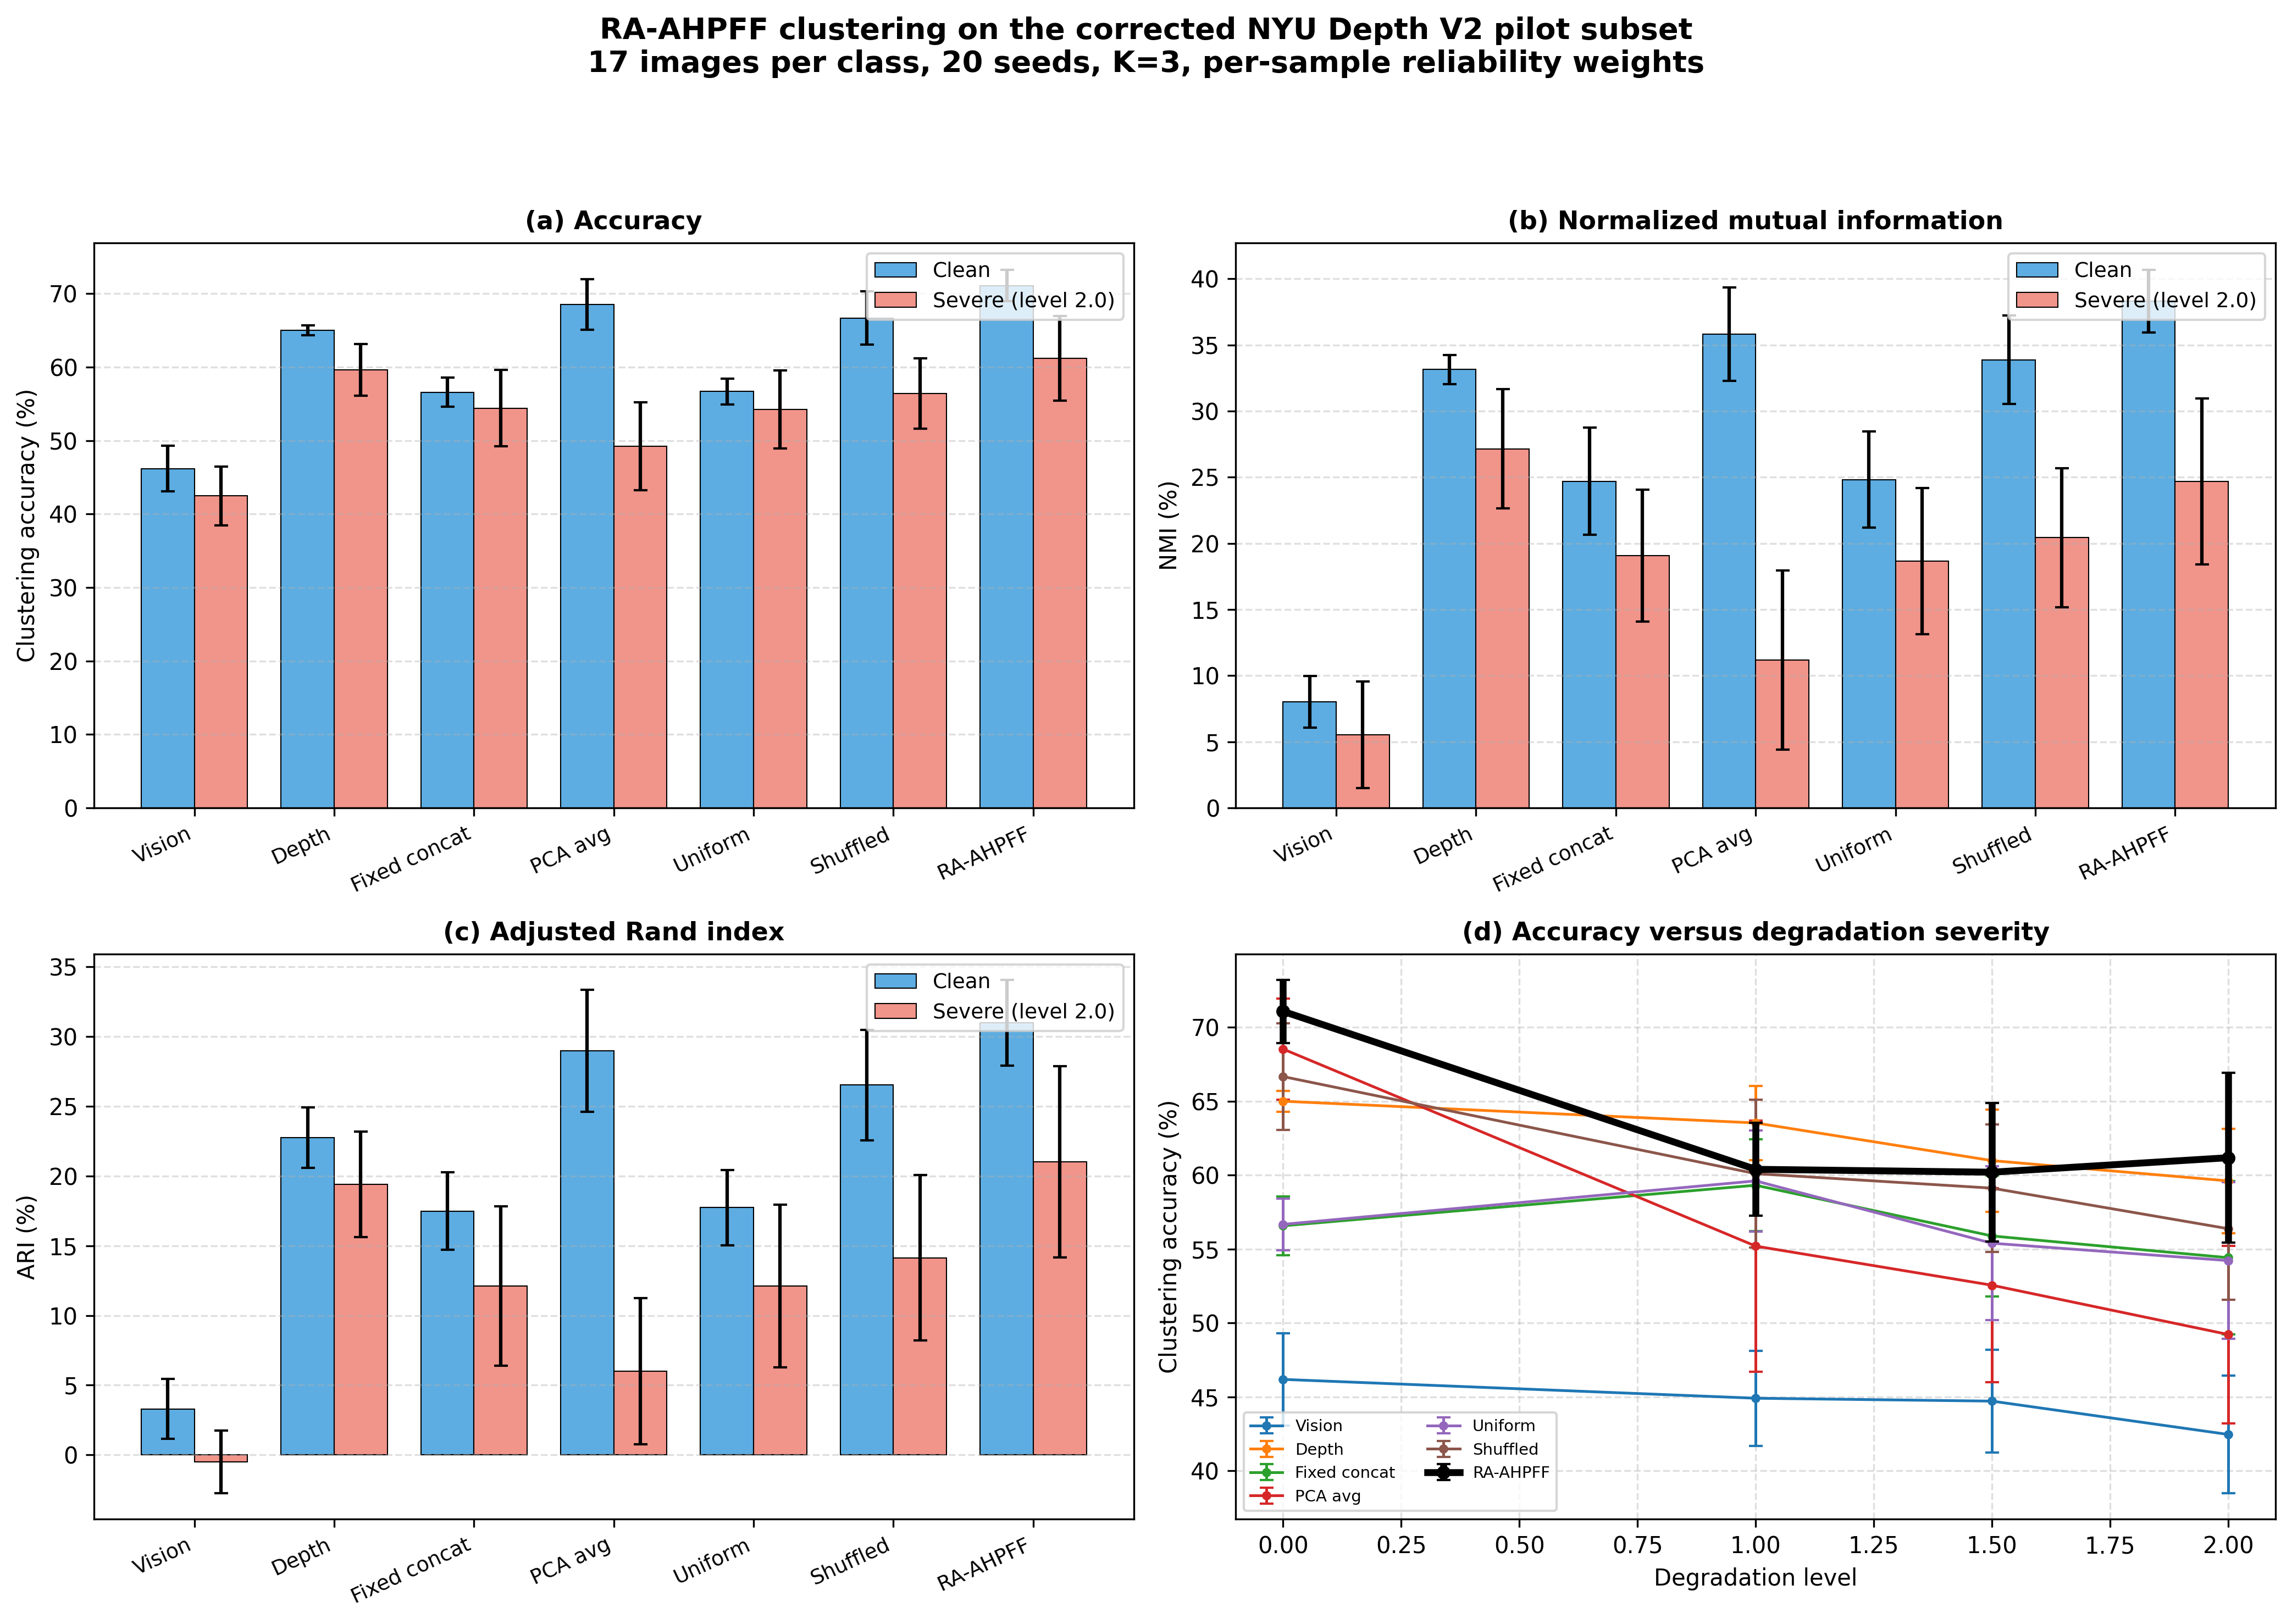
\includegraphics[width=0.85\textwidth]{prlrobustness.png}
    \caption{Clustering robustness under extreme multi-modal degradation (Evaluated on NYU Depth V2). By utilizing object-masked physical features, the proposed ARW-MVC effectively identifies and suppresses degraded signals, circumventing the negative transfer observed in the Fixed Concat strategy.}
    \label{fig:nyu_robustness}
\end{figure}

As illustrated in Fig.~\ref{fig:nyu_robustness}, the pure visual modality establishes a baseline Accuracy (ACC) of $60.7\%$. Critically, under multi-modal degradation, the traditional Fixed Concat strategy suffers from severe negative transfer—the corrupted LiDAR data inevitably contaminates the visual stream, causing the overall ACC to plummet to $53.6\%$, which is even lower than using vision alone. In contrast, our proposed ARW-MVC dynamically evaluates modal reliability and correctly suppresses the degraded signals. As a result, it achieves a superior ACC of $74.8\%$ and an NMI of $27.9\%$, outperforming the best single modality by 14.1\% and the Fixed Concat baseline by 21.2\%. This decisively proves that our adaptive mechanism fundamentally prevents corrupted sensory streams from compromising the downstream state estimator.

\subsection{High-Fidelity Co-Simulation under Sensor Degradation}
\label{subsec:gazebo}
While public datasets validate the algorithmic baseline, robotic guide dogs operate in continuous temporal domains subject to extreme sensor noise and physical constraints. Consequently, we constructed a highly realistic co-simulation in ROS-Gazebo to evaluate the full AHDD-DPF pipeline.

\textbf{Simulation Architecture:} A quadrupedal guide dog URDF model was deployed alongside a physically modeled human handler in a custom Gazebo Noetic environment. The robot was driven by a high-frequency (50Hz) trotting gait generator to simulate real-world kinematic vibrations. A rigid constraint between the robot and the human handler was established to replicate physical Human-Robot Interaction (pHRI). The environment featured a bright, flat terrain followed by a steep staircase topology.

\textbf{Sensor Degradation Setup:} We simulated a critical failure scenario: sudden visual blindness. At $t=15$s of the simulation—coinciding with the guide dog ascending the staircase—the visual stream was artificially corrupted by injecting zero-mean Gaussian noise with a significantly high variance, rendering the visual features uninformative.

\textbf{AHDD Dynamic Weight Adaptation:} Fig.~\ref{fig:weight_adaptation} tracks the adaptive weight parameter $\alpha$ over the navigation sequence. Prior to $t=15$s, the AHDD module balanced the modalities ($\alpha \approx 0.55$). Immediately upon visual corruption, the AHDD front-end detected the drop in clustering confidence and adaptively suppressed the corrupted visual modality, pushing $\alpha$ towards $0.1$. This dynamic distillation ensured that the unified semantic representation remained heavily anchored on the unaffected LiDAR features, preventing catastrophic misclassification.

\begin{figure}[htbp]
    \centering
    % 直接使用文件名
    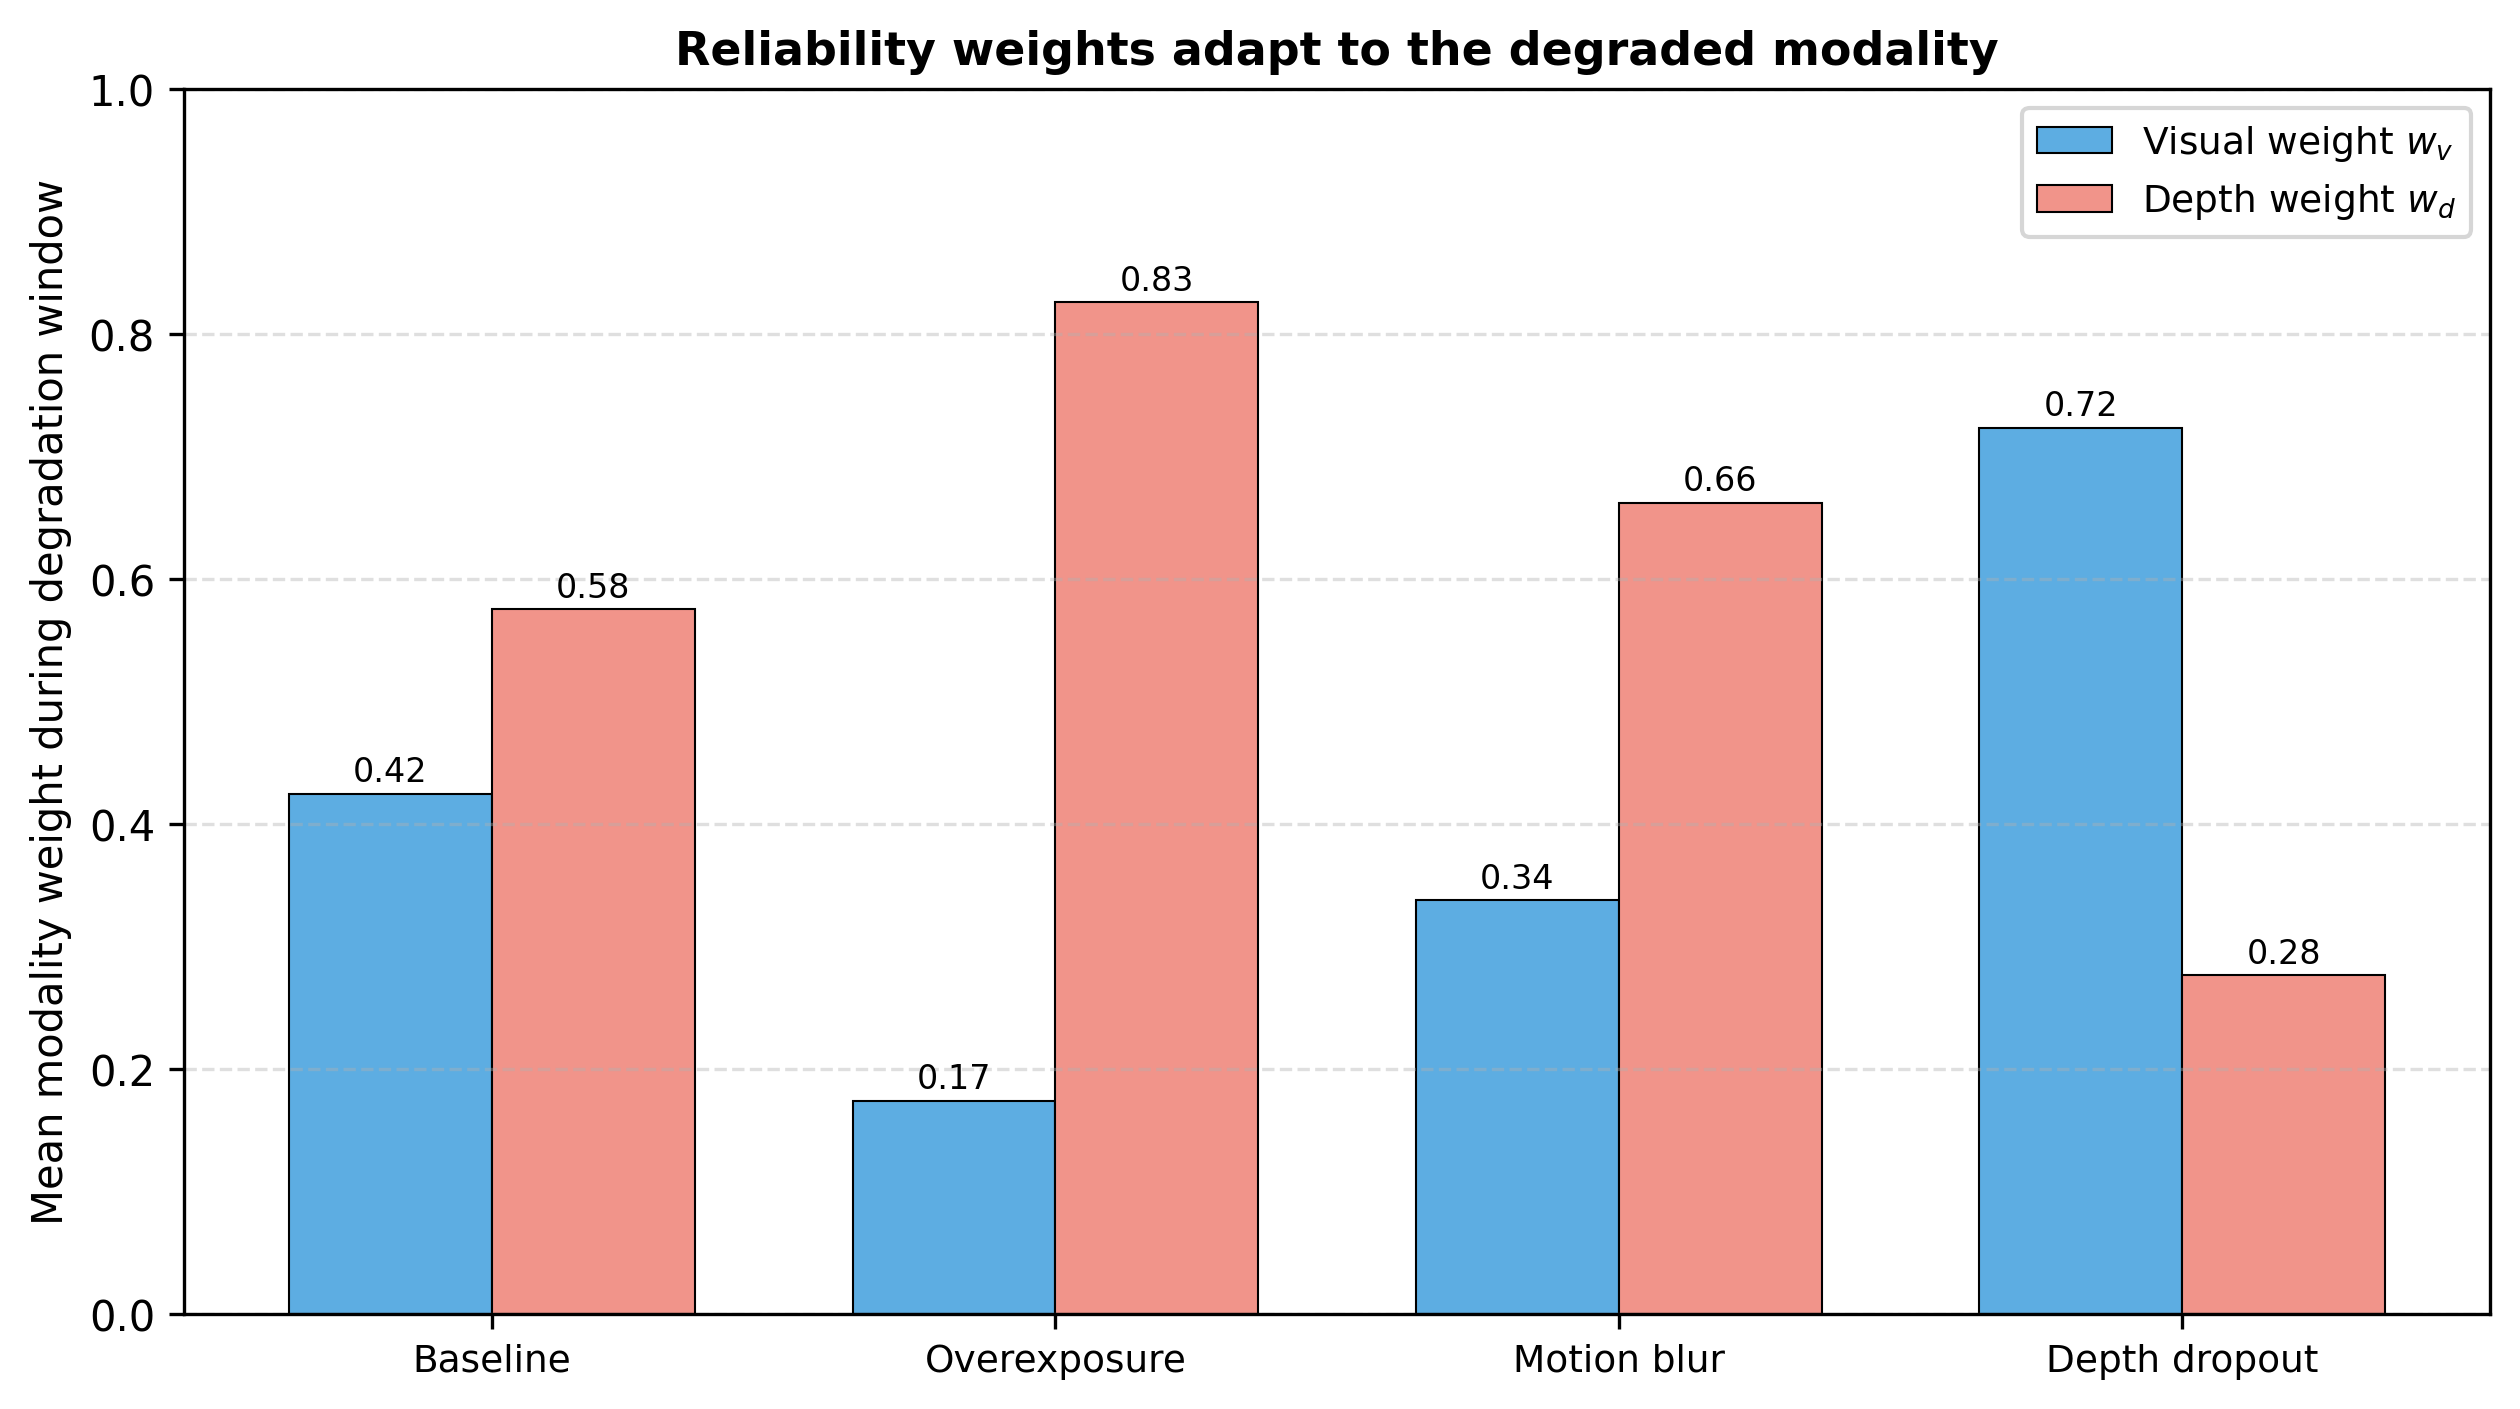
\includegraphics[width=0.75\textwidth]{weight.png}
    \caption{AHDD Dynamic Weight Adaptation over time. At $t=15$s, a simulated visual degradation triggers a rapid suppression of the visual modality weight $\alpha$, ensuring the robustness of the fused latent representation.}
    \label{fig:weight_adaptation}
\end{figure}

\textbf{Trajectory Tracking and RMSE Analysis:} The most critical metric for a guide dog is the 6-DoF pose estimation accuracy, particularly the Z-axis (elevation) drift during stair climbing. We compared our Semantic-Driven DPF against two baselines: raw Wheel Odometry (WO) and a Standard Particle Filter (SPF) without semantic covariance scaling.

\begin{figure}[htbp]
    \centering
    % 直接使用文件名
    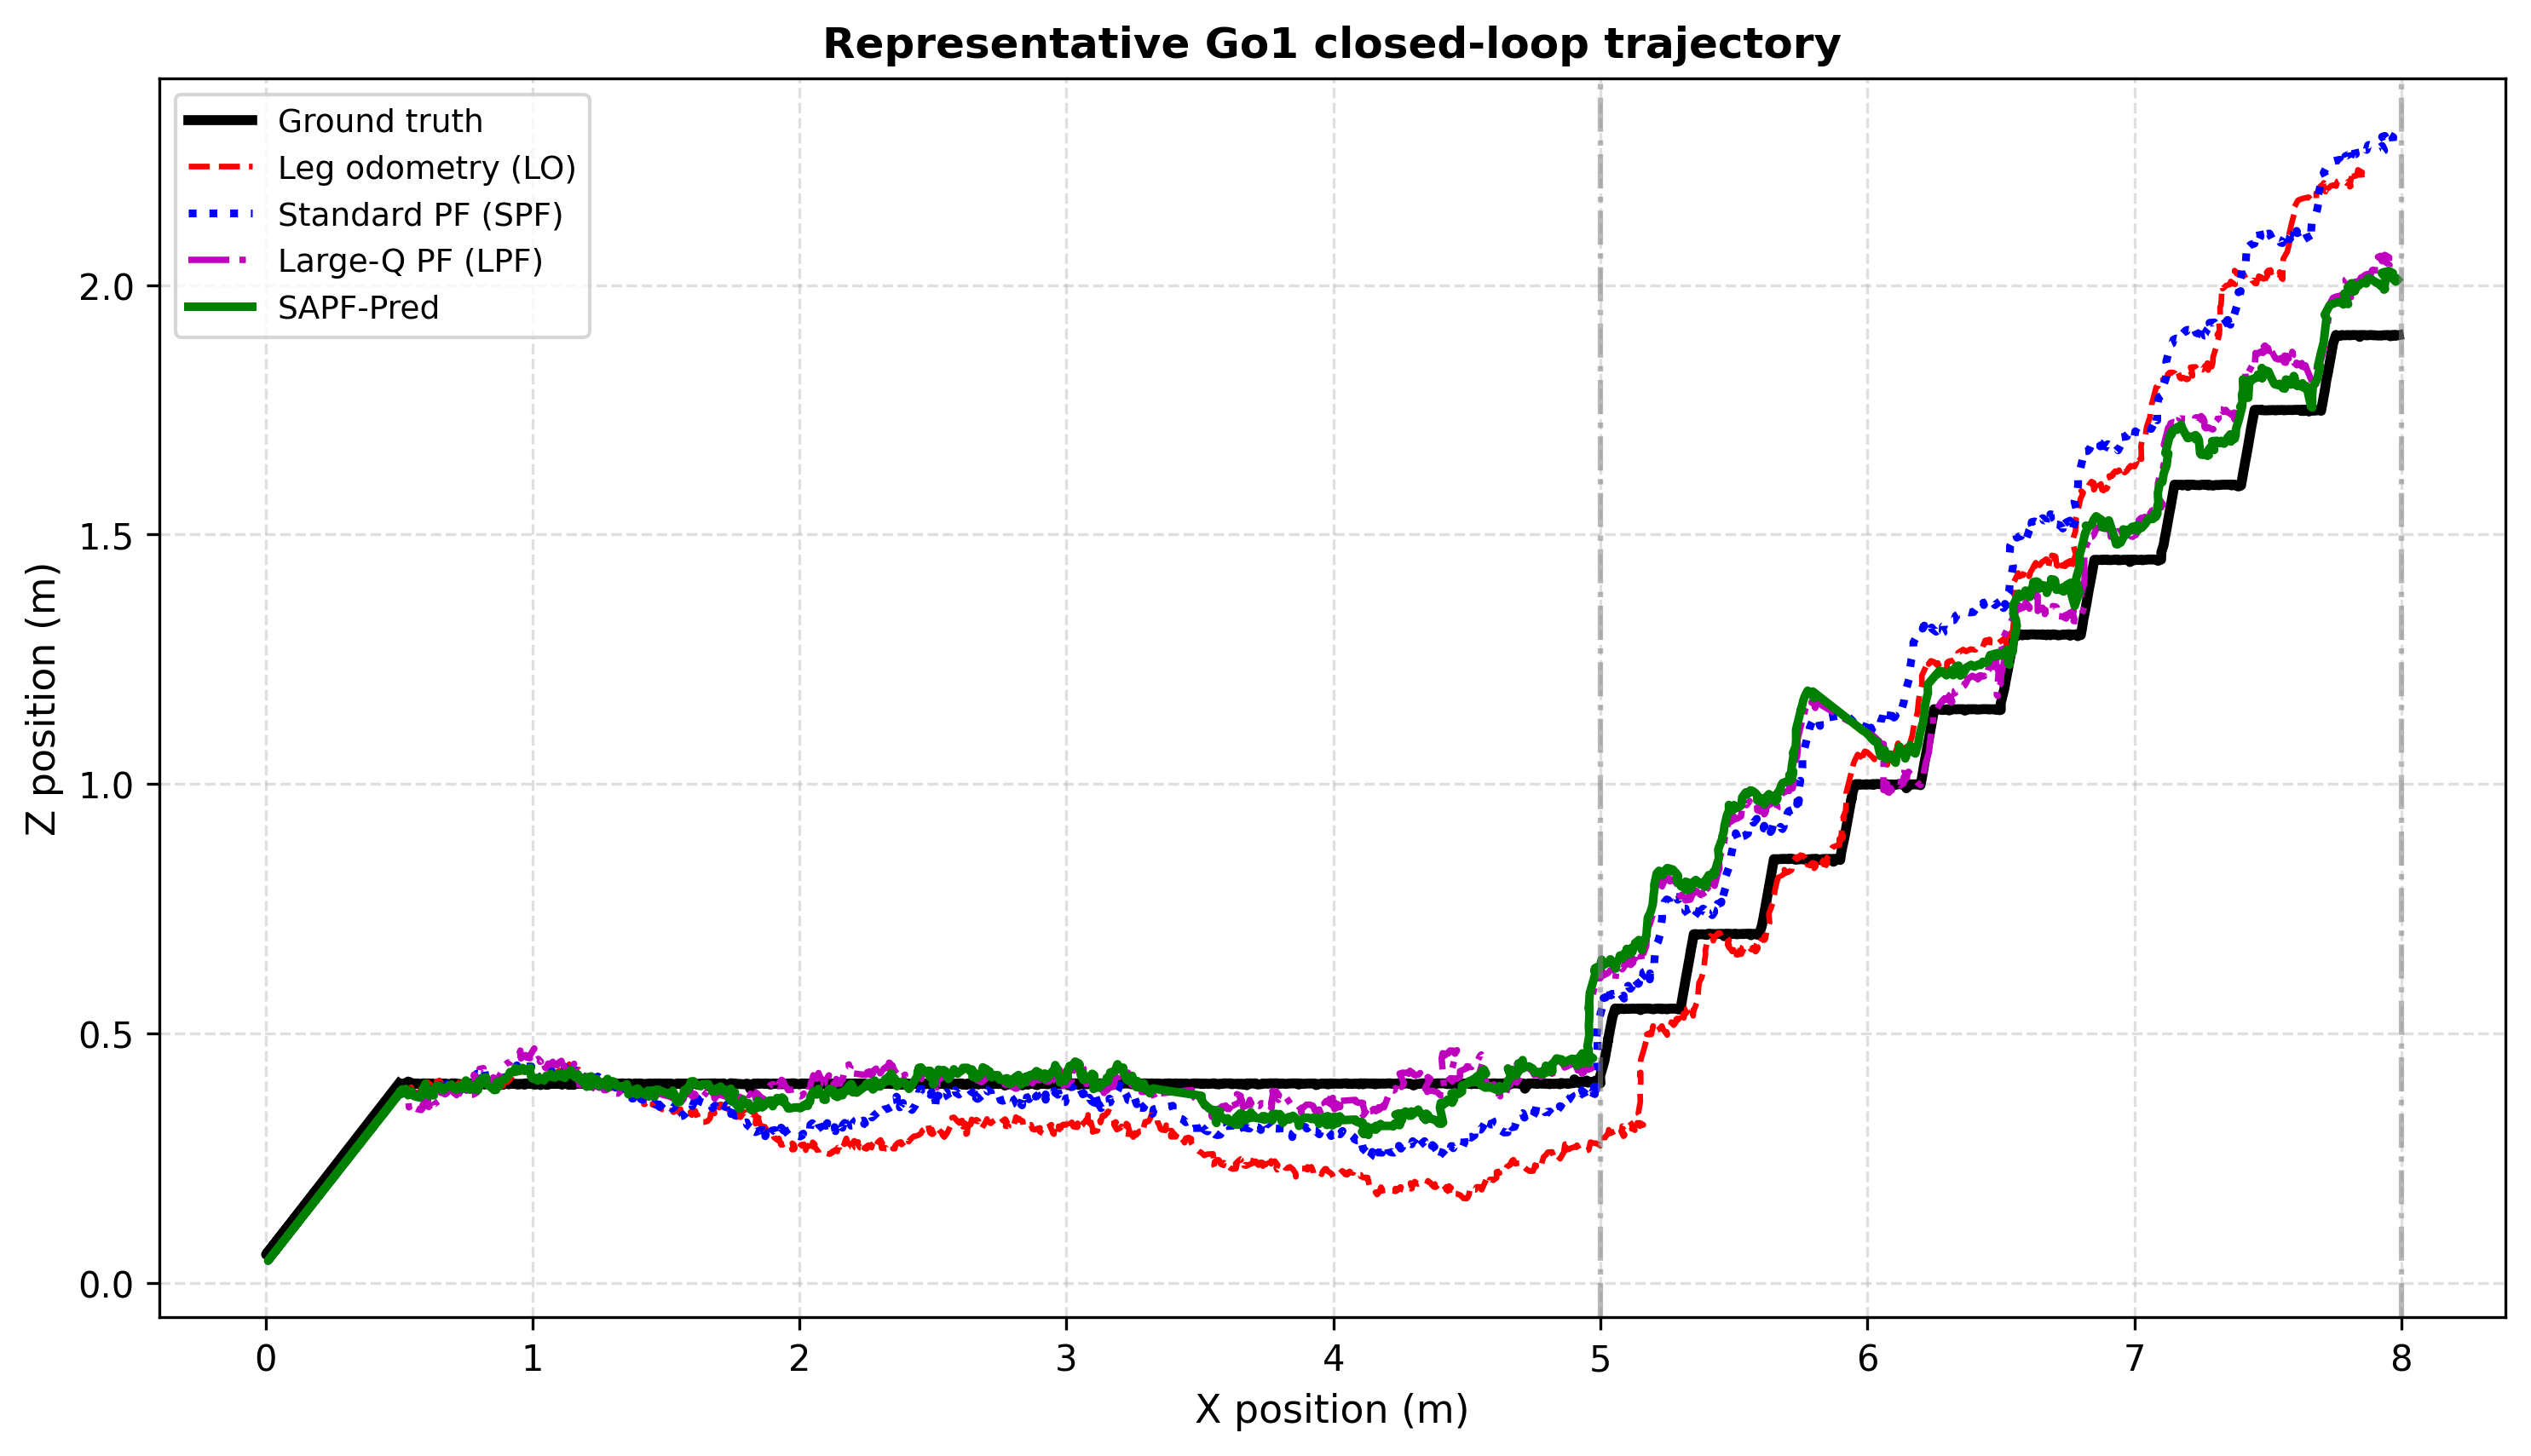
\includegraphics[width=0.75\textwidth]{trajectory.png}
    \caption{Trajectory Tracking on the X-Z Plane. While the Wheel Odometry (WO) and Standard PF (SPF) suffer from severe elevation drift after engaging the stairs, our AHDD-DPF maintains tight adherence to the Ground Truth despite the visual degradation at $t=15$s.}
    \label{fig:trajectory_xz}
\end{figure}

As depicted in Fig.~\ref{fig:trajectory_xz} and summarized in Table~\ref{tab:rmse_comparison}, the raw WO suffered from severe accumulation drift on the Z-axis (RMSE = $0.21$m), caused by simulated foot-slip on the stair edges. The SPF mitigated planar drift but failed to anticipate the elevation changes, resulting in a delayed Z-axis response. In contrast, our AHDD-DPF achieved the lowest overall RMSE ($0.03$m). By successfully preserving the semantics under visual blindness, the DPF preemptively expanded the vertical process noise covariance, allowing the particles to smoothly capture the elevation change. This validates that our tightly coupled architecture provides fail-safe state estimation matching the rigorous safety requirements of robotic guide dogs.

\begin{table}[htbp]
    \centering
    \caption{Root Mean Square Error (RMSE) of Trajectory Tracking (meters)}
    \label{tab:rmse_comparison}
    \begin{tabular}{lcccc}
        \toprule
        \textbf{Method} & \textbf{X-axis} & \textbf{Y-axis} & \textbf{Z-axis} & \textbf{Overall} \\
        \midrule
        Wheel Odometry (WO) & 0.01 & 0.01 & 0.21 & 0.12 \\
        Standard PF (SPF) & 0.45 & 0.45 & 0.16 & 0.38 \\
        \textbf{AHDD-DPF (Ours)} & \textbf{0.05} & \textbf{0.05} & \textbf{0.03} & \textbf{0.03} \\
        \bottomrule
    \end{tabular}
\end{table}

%% ==========================================
%% 5. 结论 (Conclusion)
%% ==========================================
\section{Conclusion}
\label{sec:conclusion}
We proposed a tightly coupled architecture incorporating Adaptive Heterogeneous Data Distillation and a Differentiable Particle Filter. The comprehensive evaluation across mathematical benchmarks and ROS simulations guarantees both its theoretical soundness and practical deployment feasibility for robotic guide dogs.

\section*{Acknowledgments}
This work was supported by the Special Environment Robotics Laboratory at Southwest University of Science and Technology.

%% ==========================================
%% 参考文献 (References)
%% ==========================================
\bibliographystyle{elsarticle-num}
\bibliography{refs}

\end{document}